%!TEX root = ../main.tex

\chapter{Digitalizzazione di audio analogico} \label{chp:digitalizzazione}

Preservare dall'oblio il proprio patrimonio culturale è sicuramente una delle necessità più antiche dell'uomo.

Al contrario della conservazione passiva, che consiste nella sola salvaguardia dei documenti nella loro dimensione fisica; l'unica soluzione per preservare a lungo termine il materiale analogico è la digitalizzazione, ovvero una conservazione di tipo attivo.
Tra il materiale da digitalizzare, quello audio-visivo è sicuramente uno dei più complicati per via della necessità di preservare sia il suo stato e la sua performance attuali, seppur il documento sia rovinato dal tempo o dall'usura, compreso di tutte le informazioni accessorie, sia di disporre di una copia cosiddetta "di accesso" in maniera tale da essere riprodotta agilmente con tecnologie odierne.

Molte organizzazioni quali archivi, librerie e musei non hanno ancora messo in pratica misure atte a preservare a tempo indeterminato il loro patrimonio culturale e ciò si verifica non solo nelle nazioni a più basso sviluppo umano come quelle dell'Africa subsahariana \cite{rakemaneChallengesManagingPreserving2021}, ma anche in nazioni a più alto indice di sviluppo umano come l'Italia \cite{raimoDigitalizationCulturalIndustry2022} presentando criticità non del tutto dissimili come, per esempio, la mancanza di fondi per via della poca importanza riposta nella causa. % anche loro hanno trovato l'istituzione ed implementazione di politiche di conservazione come soluzione

I musei che negli anni e soprattutto con l'avvento del COVID-19 si sono dovuti adeguare introducendo la tecnologia digitale dapprima nelle loro strutture per migliorare l'esperienza dei visitatori e poi in rete creando delle mostre virtuali generando anche maggiori visite ed incassi \cite{raimoDigitalizationCulturalIndustry2022}, ora possono sfruttare la digitalizzazione con lo scopo accessorio di creare nuove esperienze online.
Questo sforzo è anche in linea con le raccomandazioni dell'UNESCO \cite{unescoRecommendationConcerningProtection} in riferimento all'importanza della tecnologia in ambito educativo e culturale.


% TODO mostrare meglio la differenziazione tra audio e generico
\section{Filologia e Fedeltà} \label{sec:filologia-fedeltà}
La maniera più basilare di procedere alla digitalizzazione è registrare soltanto l'informazione primaria ovvero, nel caso di un prodotto sonoro, il segnale audio.
Per digitalizzare, invece, il prodotto in maniera filologicamente corretta è necessario memorizzare anche le informazioni ausiliarie come le annotazioni sul contenitore o sul supporto, i rumori presenti sul sistema di registrazione originale, le alterazioni fisiche del supporto, il marchio e modello del supporto ed altri metadati, oltre alla storia del tramandamento del documento (archiviazione, duplicazione, ecc.) \cite[p. 59]{prettoComputingMethodologiesSupporting2018}.

Per ottenere il massimo livello di aderenza alla realtà: la fedeltà, si deve assicurare, oltre che una riproduzione audio fedele, anche una simulazione dell'esperienza di interazione col dispositivo di riproduzione ed una riproduzione dei metadati e delle informazioni contestuali come ad esempio mostrato nel capitolo 3 di \textcite{fantozziTapeMusicArchives2017}.

In certi casi può essere utile operare delle modifiche alla traccia digitalizzata o ad una sua copia nel caso in cui ci siano degli errori o delle corruzioni nel supporto originario o nella digitalizzazione. Tali modifiche possono essere correttive atte a ripristinare la corretta riproduzione secondo i canoni dettati dalla filologia, oppure possono essere utili a creare una copia di accesso a discapito della fedeltà assoluta.


\section{Digitalizzazione manuale e automatizzazione} \label{sec:digitalizzazione-man-vs-auto}
Il trasferimento da analogico a digitale dipende ancora dall'esperienza dell'operatore (dalle sue valutazioni e scelte se intervenire o meno), ciò può comportare l'introduzione di errori indesiderati causati dalla perdita di attenzione umana in seguito a numerose ore di lavoro con riflessi negativi sul valore dei documenti creati e sull'affidabilità dell'intera collezione.
Per questo motivo è importante l'automatizzazione delle attività ripetitive in modo da minimizzare tali errori, ma anche da tagliare i costi e risparmiare tempo di lavoro \cites[cap. 2.1]{fantozziTapeMusicArchives2017}[es. 5]{mpaiApplicationNoteRev}.


\section{Il Centro di Sonologia Computazionale ed il suo metodo di digitalizzazione} \label{sec:csc-digitalizzazione}
Il \ac{CSC} del \ac{DEI} dell'Università di Padova, che da circa 50 anni opera nella ricerca in ambito acustico \cite{canazzaGestureMusicComputer2022}, è uno dei poli più all'avanguardia per quanto concerne la digitalizzazione di supporti musicali, nello specifico di nastri magnetici a bobina aperta (open reel tape) ed è uno dei maggiori sostenitori dell'utilizzo di automazioni nel processo di trasporto da analogico a digitale.

Dato che documentare il processo che ha generato la copia di conservazione è importante nel campo dell'audio, visto che il supporto originario potrebbe diventare irrecuperabile in futuro, il \ac{CSC} negli anni, collaborando con diversi archivi digitali, si è impegnato a sviluppare una tecnica di digitalizzazione "filologicamente informata" e di documentare la procedura in maniera accurata, verificabile ed oggettiva con l'obiettivo di creare uno standard.

L'innovazione principale in questo protocollo è la registrazione video del nastro magnetico contemporaneamente alla registrazione della traccia audio: viene effettuata la ripresa ai fini di catturare le immagini del nastro in corrispondenza della testina di registrazione ed in corrispondenza del capstan, le regioni interessate si possono trovare in figura \ref{fig:tape-areas}.

\begin{figure}[h]
    \centering
    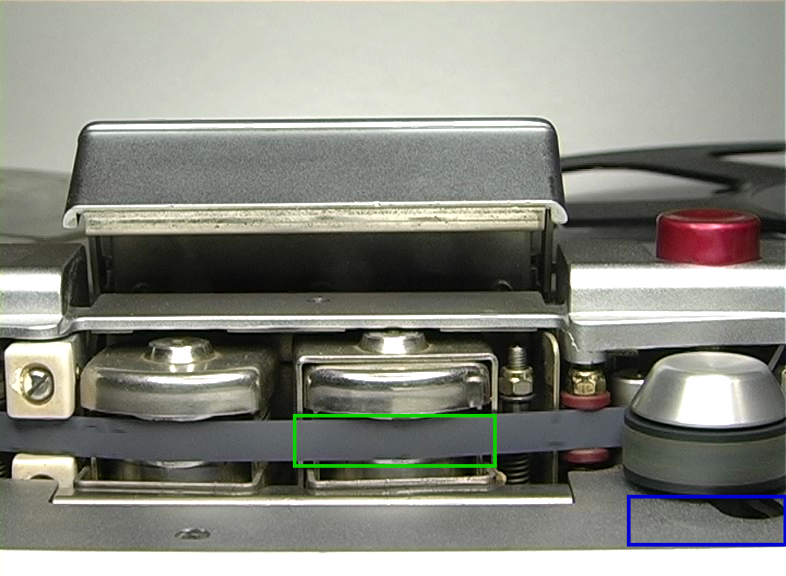
\includegraphics[width=\textwidth]{tape_areas.png}
    \caption{Regioni di interesse sotto alla testina di registrazione ed al capstan \cite{russoEnhancingPreservationRestoration}}
    \label{fig:tape-areas}
\end{figure}

La porzione vicina al capstan\footnote{Riquadro blu in figura \ref{fig:tape-areas}} serve ad individuare l'inizio della registrazione in quanto esso trasla verso il nastro nel momento in cui il motore viene azionato; mentre la sezione davanti alla testina di registrazione\footnote{Riquadro verde in figura \ref{fig:tape-areas}} serve ad individuare, tramite tecniche di intelligenza artificiale, tutte le alterazioni del retro nel nastro che, da ora in poi, chiameremo "irregolarità"; alcuni esempi sono giunzioni, scritte e parti visivamente danneggiate o rovinate, vedi figura \ref{fig:nastro-irrs}.
Questi sono parte dei metadati citati all'inizio di questa sezione.
L'utilità di raccogliere tali dati legati alla traccia audio è quella, oltre che di catturare il documento nella sua essenza più completa, anche di poter ricollegare la performance di una qualsiasi porzione della traccia audio ad un'eventuale irregolarità sul nastro ed eventualmente agire di conseguenza.

\begin{figure}
     \centering
     \begin{subfigure}{0.45\textwidth}
         \centering
         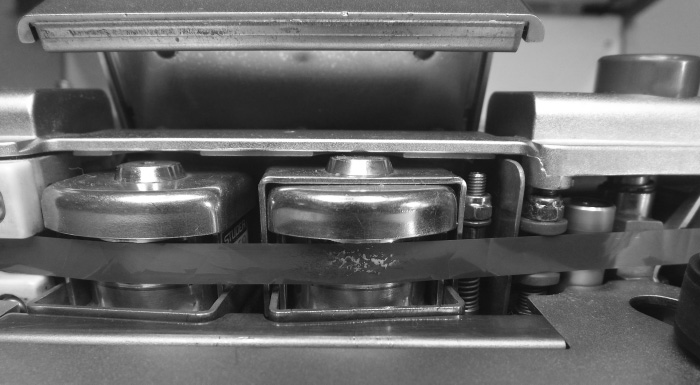
\includegraphics[width=\textwidth]{nastro_rovinato.png}
         \caption{Porzione di nastro rovinata \cite{prettoComputingMethodologiesSupporting2018}}
         \label{fig:nastro-rovinato}
     \end{subfigure}
     \hfill
     \begin{subfigure}{0.45\textwidth}
         \centering
         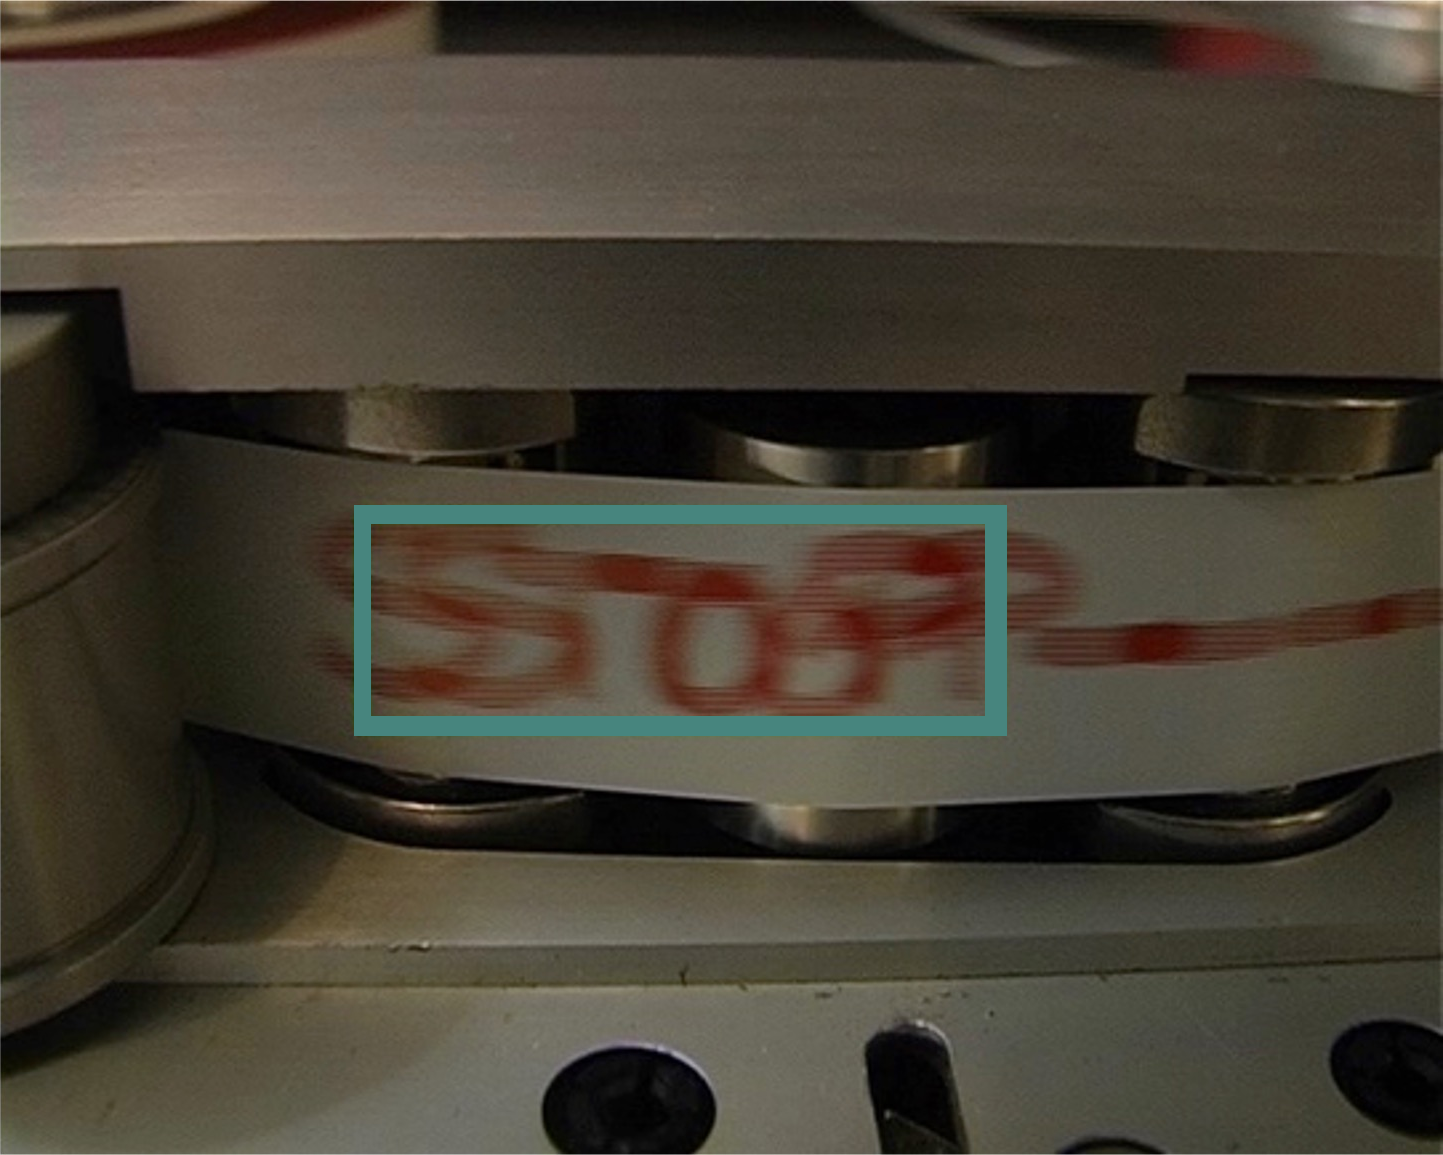
\includegraphics[width=\textwidth]{nastro_testo.png}
         \caption{Testo su nastro \cite{canazzaGestureMusicComputer2022}}
         \label{fig:nastro-testo}
     \end{subfigure}
        \caption{Alcuni esempi di irregolarità}
        \label{fig:nastro-irrs}
\end{figure}

La procedura creata dal \ac{CSC} prevede anche una gestione di tracce audio catturate a velocità o equalizzazione incorrette:

La velocità, misurata in pollici per secondo (\textit{inches per second}, ips in inglese), è solitamente impostata a sottomultipli binari di \qty{30}{ips} e viene regolata in base alla qualità di registrazione ed alla durata di un nastro che l'artista ha voluto ottenere, in generale maggiore è la velocità, maggiore sarà la qualità di registrazione e minore la durata del nastro.
Può accadere che nello stesso nastro digitalizzato siano presenti tracce a velocità diverse ed alcuni motivi potrebbero essere le aggiunte di altro nastro, registrato diversamente, per eseguire del montaggio, oppure la diminuzione di velocità all'avvicinarsi della fine del nastro in maniera tale da concludere la performance senza dover utilizzare un nuovo supporto, oppure ancora la registrazione di più performance scorrelate tra loro all'interno stesso nastro.

Per quanto riguarda l'equalizzazione invece, le curve di equalizzazione\footnote{L'equalizzazione è una tecnica di filtraggio che permette di variare l'ampiezza delle frequenze di un segnale audio; una curva di equalizzazione è ottenuta dalla combinazione dei risultati delle due curve $N(DB)=10 \log(1 + \frac{1}{4 \pi^2 f^2 t_2^2}) - 10 \log(1+4\pi^2 f^2 t_1^2)$ dove $f$ è la frequenza in \unit{\Hz} e $t_1$ e $t_2$ sono costanti di tempo in secondi.} solitamente sono quelle dettate dagli standard \acs{CCIR}, utilizzato in Europa, e \acs{NAB}, utilizzato in USA.

Il CSC utilizza ancora una volta un modello di machine learning allenato a riconoscere in porzioni di audio di \qty{500}{\ms} se la velocità e la curva di equalizzazione impostate al momento del trasferimento da analogico a digitale sono corrette ed a classificarle con le velocità ed equalizzazione corrette; per fare ciò si da in pasto al modello pre-allenato il rumore estrapolato dai silenzi presenti nell'interezza della traccia audio ed i relativi primi 13 coefficienti spettrali mel (\acfi{MFCC}\footnote{I coefficienti spettrali mel sono una rappresentazione del segnale acustico, solitamente sono utilizzati per rappresentare le caratteristiche generali del segnale acustico e vengono spesso utilizzati in applicazioni di riconoscimento del parlato e recupero di informazioni musicali; sono calcolati a partire dal segnale audio su cui viene applicata la trasformata di Fourier con cui si calcola la potenza dello spettro e la si riscala con la scala mel (una scala basata sulla percezione dell'altezza del suono), dopodiché vengono applicati il logaritmo e la trasformata discreta del coseno; i coefficienti sono le ampiezze dello spettro risultante.}).
% TODO scrivere successo 93,7% di aa?
